\section{Auswertung}
\label{sec:Auswertung}
In diesem Versuch stehen drei Spiegel als Enden des Resonators zur Verfügung. Ein Spiegel ist ein konkaver Auskopplungsspiegel (OC) mit einem Radius 
$r_1 = \qty{1400}{\milli\metre}$, welcher immer verwendet werden muss, da hierüber das Licht ausgekoppelt wird.
Dazu können ein weiterer konkaver Spiegel mit Radius $r_2 = \qty{1400}{\milli\metre}$ (Konfiguration 1) und ein flacher Spiegel mit $r_2 = \infty$ (Konfiguration 2) verwendet werden.
\subsection{Überprüfung der Stabilitätsbedingung}
Zuerst wird die Stabilitätsbedingung \eqref{eq:g1g2} überprüft.
Die Theoriekurven der Stabilitätsbedingung nach \autoref{eq:g1g2} sind für beide Spiegelkonfigurationen in \autoref{fig:stability} zu sehen.
\begin{figure}
  \centering
  \includegraphics[width = .8\textwidth]{stability.pdf}
  \caption{Stabilitätsbedingung für die verwendeten Spiegelkonfigurationen.}
  \label{fig:stability}
\end{figure}
Für die erste Spiegelkonfigurationen ist eine Stabilität des Laserbetriebs bis $\qty{2.8}{\metre}$ zu erwarten, für die zweite Konfiguration sind es $\qty{1.4}{\metre}$.
In \autoref{tab:stability} ist die maximal gemessene Laserleistung gegen die Resonatorlänge aufgetragen. Für beide Konfigurationen bestätigt sich die theoretische 
Stabilitätsbedingung, wobei der Messbereich nur bis zu einer Resonatorlänge von $\qty{2}{\metre}$ reicht.
Für alle weiteren Messungen wird die erste Spiegelkonfigurationen (konkav, konkav) verwendet.
\begin{table}
  \centering
  \aboverulesep=0ex % Solution part 1 of 3
  \belowrulesep=0ex % Solution part 1 of 3
  \caption{Messdaten zur Überprüfung der Stabilitätsbedingung für beide Spiegelkonfigurationen.}
  \label{tab:stability}
  \begin{tabular}{S[table-format = 3.0] S[table-format = 1.1] | S[table-format = 3.1] S[table-format = 1.1]}
    %\toprule
    \multicolumn{2}{c}{$r_2 = \qty{1400}{\milli\metre}$} & \multicolumn{2}{c}{$r_2 = \infty$} \\
    \midrule
    \rule{0pt}{1.1EM}
    {$L \mathbin{/} \unit{\centi\metre}$} & {$I \mathbin{/} \unit{\milli\watt}$} & {$L \mathbin{/} \unit{\centi\metre}$} & {$I \mathbin{/} \unit{\milli\watt}$}\\
    \midrule
    \rule{0pt}{1.1EM}
     50 & 3.0 &    55 & 4.8 \\
     75 & 4.0 &    70 & 2.0 \\
    100 & 2.8 &    96 & 2.4 \\
    125 & 2.7 &   120 & 4.3 \\
    150 & 2.2 &   131 & 3.2 \\
    175 & 3.3 & 134.5 & 2.7 \\
    200 & 2.0 & 137.5 & 1.0 \\
        &     &   140 & 1.0 \\
        &     &   141 &   0 \\ 
    %\bottomrule
  \end{tabular}
\end{table}

\subsection{Messung der TEM Moden}

Zur Messung der verschiedenen transversalen Moden (TEM) wird der Tungstendraht in den Laserstrahl gespannt.
In \autoref{fig:TEM_Modes} sind verschiedene observierte Moden abgebildet.

\begin{figure}
  \begin{subfigure}{.45\textwidth}
    \centering 
    \includegraphics[width = \textwidth]{content/pics/TEM01.jpg}
    \caption{$\text{TEM}_{10}$}
    \label{fig:TEM01_pic}
  \end{subfigure}
  \hfill
  \begin{subfigure}{.45\textwidth}
    \centering 
    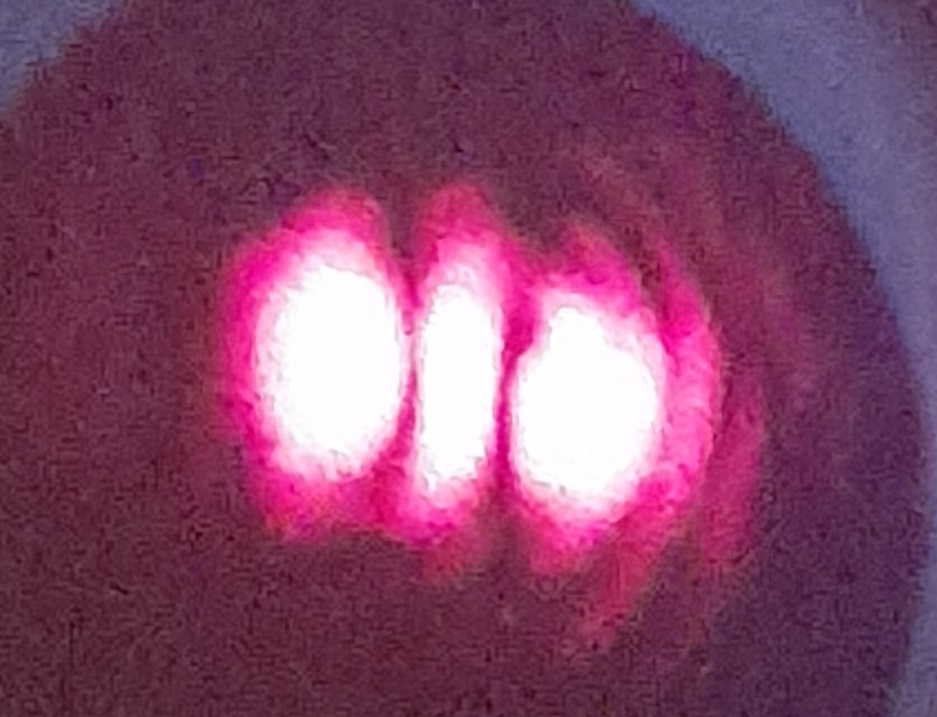
\includegraphics[width = \textwidth]{"content/pics/TEM02.jpg"}
    \caption{$\text{TEM}_{20}$}
    \label{fig:TEM02_pic}
  \end{subfigure}
  \caption{Verschiedene TEM Moden des Lasers.}
  \label{fig:TEM_Modes}
\end{figure}
Es wird die Intensitätsverteilung der $\text{TEM}_{00}$ und $\text{TEM}_{10}$ Moden vermessen. Die Messdaten können \autoref{tab:TEM} entnommen werden.
\begin{table}[H]
  \centering
  \aboverulesep=0ex % Solution part 1 of 3
  \belowrulesep=0ex % Solution part 1 of 3
  \caption{Messdaten der Intensitätsverteilung der $\text{TEM}_{00}$ und $\text{TEM}_{10}$ Moden.}
  \label{tab:TEM}
  \begin{tabular}{S[table-format = 2.0] | S[table-format = 1.3]  S[table-format = 1.2]}
    %\toprule
    {} & {$\text{TEM}_{00}$} & {$\text{TEM}_{10}$} \\
    \midrule
    \rule{0pt}{1.1EM}
    {$d \mathbin{/} \unit{\milli\metre}$} & {$I \mathbin{/} \unit{\micro\ampere}$} & {$I \mathbin{/} \unit{\micro\ampere}$} \\
    \midrule
    \rule{0pt}{1.1EM}
    -20 & 0.015 & 0.03 \\
    -18 & 0.021 & 0.03 \\
    -16 & 0.025 & 0.01 \\
    -14 & 0.034 & 0.01 \\
    -12 & 0.062 & 0.04 \\
    -10 & 0.28  & 0.12 \\
     -9 & 0.43  & 0.20 \\
     -8 & 0.74  & 0.31 \\
     -7 & 1.11  & 0.42 \\
     -6 & 1.53  & 0.55 \\
     -5 & 2.08  & 0.69 \\
     -4 & 2.8   & 0.73 \\
     -3 & 3.3   & 0.70 \\
     -2 & 3.7   & 0.58 \\
     -1 & 3.6   & 0.40 \\
      0 & 3.6   & 0.25 \\
      1 & 2.9   & 0.10 \\
      2 & 2.4   & 0.02 \\
      3 & 1.5   & 0.05 \\
      4 & 0.96  & 0.17 \\
      5 & 0.36  & 0.31 \\
      6 & 0.20  & 0.42 \\
      7 & 0.14  & 0.53 \\
      8 & 0.10  & 0.54 \\
      9 & 0.068 & 0.56 \\
     10 & 0.047 & 0.50 \\
     12 & 0.018 & 0.35 \\
     14 & 0.009 & 0.17 \\
     16 & 0.006 & 0.09 \\
     18 & 0.005 & 0.03 \\
     20 & 0.004 & 0.02 \\
    %\bottomrule
  \end{tabular}
\end{table}

\subsubsection{$\text{TEM}_{00}$-Mode}

Die Intensität der $\text{TEM}_{00}$-Mode folgt nach \autoref{eq:I_mn} einer Gaußverteilung, weshalb eine Funktion
\begin{equation*}
  I(x) = I_0 \text{exp}\left[-(x-x_0)^2/\omega^2\right]
\end{equation*}
mittels \textit{scipy} \cite{scipy} an die Messdaten gefitted wird.
Der resultierende Fit ist in \autoref{fig:TEM00} zu sehen.
\begin{figure}[H]
  \centering
  \includegraphics[width = .8\textwidth]{TEM00.pdf}
  \caption{Messdaten der Intensitätsverteilung der $\text{TEM}_{00}$-Mode und Fit mittels \textit{scipy} \cite{scipy}.}
  \label{fig:TEM00}
\end{figure}

Die Fitparameter ergeben sich zu 
\begin{align*}
  I_0 &= \qty{3.74 +- 0.05}{\micro\ampere} \\
  x_0 &= \qty{-1.47 +- 0.05}{\milli\metre} \\
  \omega &= \qty{4.80 +- 0.07}{\milli\metre}.
\end{align*}

\subsubsection{$\text{TEM}_{10}$-Mode}

Für die $\text{TEM}_{10}$-Mode wird die Funktion
\begin{equation*}
  I(x) = 8I_0\frac{(x-x_0)^2}{\omega^2} \text{exp}\left[-(x-x_0)^2/\omega^2\right]
\end{equation*}
an die Messdaten gefitted.
\begin{figure}[H]
  \centering
  \includegraphics[width = .8\textwidth]{TEM01.pdf}
  \caption{Messdaten der Intensitätsverteilung der $\text{TEM}_{10}$-Mode und Fit mittels \textit{scipy} \cite{scipy}.}
  \label{fig:TEM01}
\end{figure}
Die Fitparameter lauten
\begin{align*}
  I_0 &= \qty{0.22 +- 0.005}{\micro\ampere} \\
  x_0 &= \qty{2.30 +- 0.09}{\milli\metre} \\
  \omega &= \qty{6.12 +- 0.09}{\milli\metre}.
\end{align*}
Die Messdaten und der resultierende Fit sind in \autoref{fig:TEM01} abgebildet.
\subsection{Polarisation des Lasers}
Zur Bestimmung der Polarisation des Laserstrahls werden die in \autoref{tab:polarisation} gelisteten Messdaten verwendet.
\begin{table}
  \centering
  \aboverulesep=0ex % Solution part 1 of 3
  \belowrulesep=0ex % Solution part 1 of 3
  \caption{Messdaten zur Bestimmung der Polarisation des Laserstrahls.}
  \label{tab:polarisation}
  \begin{tabular}{S[table-format = 3.0] S[table-format = 1.1] | S[table-format = 3.0] S[table-format = 1.1] | S[table-format = 3.0] S[table-format = 1.1]}
    %\toprule
    {$\theta \mathbin{/} \unit{\degree}$} & {$I \mathbin{/} \unit{\milli\watt}$} & {$\theta \mathbin{/} \unit{\degree}$} & {$I \mathbin{/} \unit{\milli\watt}$} &%
    {$\theta \mathbin{/} \unit{\degree}$} & {$I \mathbin{/} \unit{\milli\watt}$} \\
    \midrule
    \rule{0pt}{1.1EM}
      0 & 0.5 & 130 & 0.8 & 250 & 3.2 \\
     10 & 0.9 & 140 & 0.4 & 260 & 3.0 \\
     20 & 1.4 & 150 & 0.1 & 270 & 2.8 \\
     30 & 2.0 & 160 & 0.1 & 280 & 2.3 \\
     40 & 2.4 & 170 & 0.2 & 290 & 1.8 \\
     50 & 2.8 & 180 & 0.4 & 300 & 1.3 \\
     60 & 3.0 & 190 & 0.9 & 310 & 0.8 \\
     70 & 3.2 & 200 & 1.4 & 320 & 0.4 \\
     80 & 3.1 & 210 & 1.9 & 330 & 0.1 \\
     90 & 2.7 & 220 & 2.5 & 340 & 0.1 \\
    100 & 2.3 & 230 & 2.9 & 350 & 0.2 \\
    110 & 1.8 & 240 & 3.1 & 360 & 0.5 \\
    120 & 1.3 &     &     &     &     \\
    %\bottomrule
  \end{tabular}
\end{table}
Aufgrund der zu erwartenden $\pi$-Periodizität wird die Funktion 
\begin{equation*}
  I(\theta) = I_1 \cdot \text{sin}^2\left(\theta + \delta \right) + I_0
\end{equation*}
zur Modellierung der Daten verwendet. Die Daten und der resultierende Fit sind in \autoref{fig:polarisation} dargestellt.
\begin{figure}
  \centering
  \includegraphics[width = .8\textwidth]{polarisation.pdf}
  \caption{Messdaten zur Bestimmung der Polarisation des Laserstrahls und Fit mittels \textit{scipy} \cite{scipy}.}
  \label{fig:polarisation}
\end{figure}
Die Parameter des Fits bestimmen sich mittels \textit{scipy} \cite{scipy} zu 
\begin{align*}
  I_1 &= \qty{3.09 +- 0.02}{\milli\watt} \\
  \delta &= \qty{21.24 +- 0.17}{\degree} \\ %= \qty{0.37 +- 0.003}{\radian} 
  I_0 &= \qty{7 +- 1e-02}{\milli\watt}.
\end{align*}
Der Laserstrahl ist somit annähernd linear polarisiert.

\subsection{Multimoden Betrieb}
Um den Multimoden Betrieb des Lasers zu untersuchen werden die in \autoref{tab:Multimoden} aufgetragen Messdaten verwendet, welchen das Frequenzspektrum des Lasers zu verschiedenen
Resonatorlängen entnommen werden kann. Aus dem gemessenen Frequenzspektrum kann der mittlere Abstand $\symup{\Delta}f$ der Frequenzpeaks bestimmt werden, welcher ebenfalls in 
\autoref{tab:Multimoden} aufgelistet ist.
\begin{table}
  \centering
  \aboverulesep=0ex % Solution part 1 of 3
  \belowrulesep=0ex % Solution part 1 of 3
  \caption{Frequenzspektrum $[f]$ des Lasers bei verschiedenen Resonatorlängen $L$.}
  \label{tab:Multimoden}
  \begin{tabular}{c | c | l}
    %\toprule
    {$L \mathbin{/} \unit{\centi\metre}$} & $[f] \mathbin{/} \unit{\mega\hertz}$ & $\symup{\Delta}f \mathbin{/} \unit{\mega\hertz}$ \\%& {$L_\text{exp} \mathbin{/} \unit{\centi\metre}$}\\
    \midrule
    \rule{0pt}{1.1EM}
     50 &                      {304, 611, 919} & {307,50 \pm \; 0,50} \\   
     \midrule
     \rule{0pt}{1.1EM} 
     75 &           {203, 405, 604, 806, 1009} & {201,50 \pm \; 1,50} \\    
     \midrule
     \rule{0pt}{1.1EM} 
    100 & {150, 300, 454, 600, 754, 904, 1054} & {150,67 \pm \; 2,75} \\   
    \midrule
    \rule{0pt}{1.1EM}  
    125 & {124, 240, 364, 480, 600, 720, 840,} & {120,00 \pm \; 2,67} \\  
        &                    {960, 1080, 1204} &                      \\   
    \midrule
    \rule{0pt}{1.1EM}  
    150 & {101, 203, 304, 401, 503, 604, 701,} & {100,64 \pm \; 1,77} \\     
        &         {803, 904, 1005, 1106, 1208} &                      \\
    \midrule
    \rule{0pt}{1.1EM}
    175 &  {86, 176, 260, 350, 435, 518, 600,} & { 86,25 \pm \; 3,03} \\   
        &     {686, 773, 863, 949, 1031, 1121} &                      \\
    \midrule
    \rule{0pt}{1.1EM}
    200 &  {75, 154, 221, 300, 375, 450, 525,} & { 75,31 \pm \; 4,18} \\
        & {596, 670, 754, 825, 904, 980, 1054} &                      \\
  \end{tabular}
\end{table}
Es lässt sich feststellen, dass der Abstand der Frequenzpeaks invers-proportional zu der Resonatorlänge ist und mit größerer Resonatorlänge mehr Frequenzen auftreten.

\subsection{Bestimmung der Wellenlänge des Lasers}
Zuletzt wird die Wellenlänge des Lasers mittels der Interferenzbedingung bei Beugung an einem Gitter ermittelt. Dazu werden verschiedene Gitter in den Strahlengang gebracht und der 
Abstand der Beugungsmaxima auf einem Schirm gemessen. Mit \autoref{eq:lambda} lässt sich dann die Wellenlänge des Lasers berechnen.
Die Messdaten und die daraus resultierenden Wellenlängen sind in \autoref{tab:wellenlänge} aufgelistet.
\begin{table}
  \centering
  \aboverulesep=0ex % Solution part 1 of 3
  \belowrulesep=0ex % Solution part 1 of 3
  \caption{Messdaten zur Bestimmung der Wellenlänge. Zu jeder Gitterkonstanten $g$ ist der Schirmabstand $d$ und der Abstand der Maxima $n$-ter Ordnung ($d_{nn}$), 
  sowie die daraus resultierende Wellenlänge $\lambda$ angegeben.}
  \label{tab:wellenlänge}
  \begin{tabular}{S[table-format = 4.0] | S[table-format = 3.0] | S[table-format = 1.0] | S[table-format = 2.1] | S[table-format = 3.2]}
    %\toprule
    {$g \mathbin{/} \unit{\milli\metre^{-1}}$} & {$d \mathbin{/} \unit{\centi\metre}$} & {$n$} & {$d_{nn} \mathbin{/} \unit{\centi\metre}$} & {$\lambda \mathbin{/} \unit{\nano\metre}$} \\
    \midrule
    \rule{0pt}{1.1EM}
    1200 & 25  & 1 &   58 & 631.18 \\
    \midrule
    \rule{0pt}{1.1EM}
     600 & 25  & 1 & 20.5 & 632.26 \\
         &     & 2 & 59.5 & 637.98 \\
    \midrule
    \rule{0pt}{1.1EM}
     100 & 80  & 1 &   10 & 623.78 \\
         &     & 2 & 20.5 & 635.43 \\
         &     & 3 &   31 & 634.04 \\
         &     & 4 &   42 & 634.75 \\
    \midrule
    \rule{0pt}{1.1EM}
      60 & 110 & 1 & 11.5 & 652.52 \\
         &     & 2 & 22.5 & 635.89 \\
         &     & 3 & 33.5 & 627.24 \\
    %\bottomrule
  \end{tabular}
\end{table}
Es ergibt sich ein Mittelwert von 
\begin{equation*}
  \lambda = \qty{634.5 +- 7.24}{\nano\metre}.
\end{equation*}
